    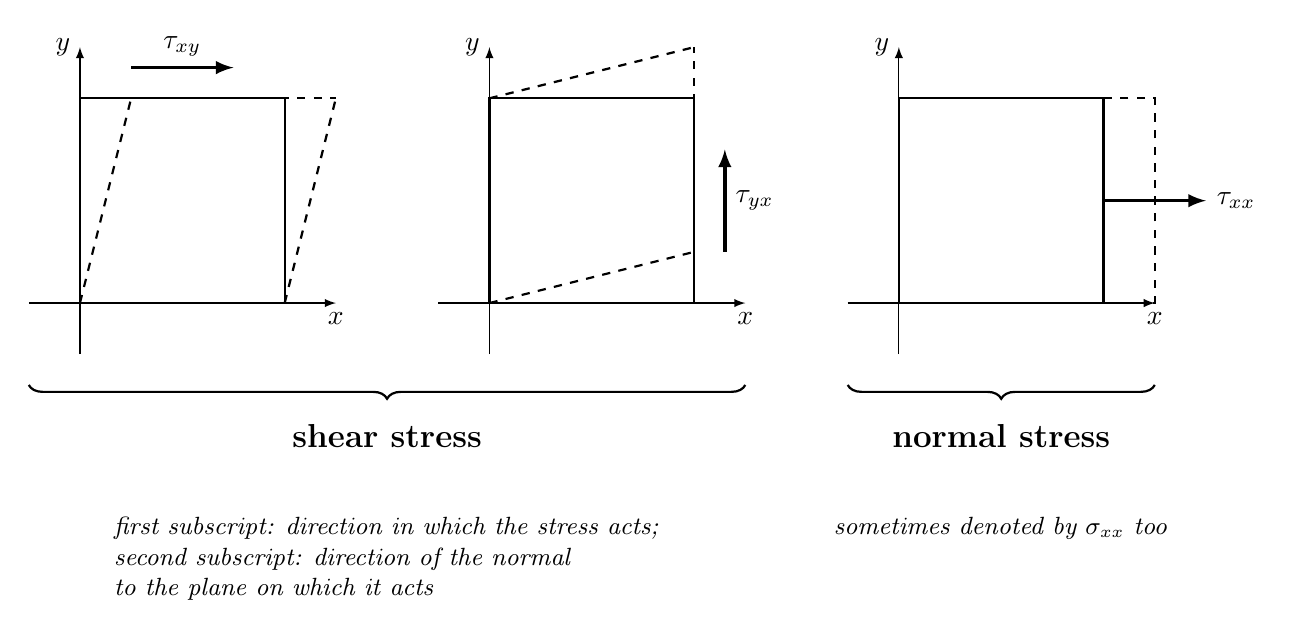
\begin{tikzpicture}[>=latex, scale=1.3]
        \tikzset{axis/.style={->, thin}, solidline/.style={thick}, dashedline/.style={thick, dashed}, forcearrow/.style={->, very thick}}
        % 1. shear stress tau_xy (acts in x on a y-face)
        \begin{scope}[shift={(0,0)}]
            \draw[axis] (-0.5,0) -- (2.5,0) node[below] {$x$};
            \draw[axis] (0,-0.5) -- (0,2.5) node[left] {$y$};
            \draw[solidline] (0,0) rectangle (2,2);
            \draw[dashedline] (0,0) -- (0.5,2);
            \draw[dashedline] (2,0) -- (2.5,2);
            \draw[dashedline] (0.5,2) -- (2.5,2);
            \draw[forcearrow] (0.5, 2.3) -- (1.5, 2.3) node[midway, above] {$\tau_{xy}$};
        \end{scope}
        % 2. shear stress tau_yx (acts in y on an x-face)
        \begin{scope}[shift={(4,0)}]
            \draw[axis] (-0.5,0) -- (2.5,0) node[below] {$x$};
            \draw[axis] (0,-0.5) -- (0,2.5) node[left] {$y$};
            \draw[solidline] (0,0) rectangle (2,2);
            \draw[dashedline] (0,0) -- (2,0.5);
            \draw[dashedline] (0,2) -- (2,2.5);
            \draw[dashedline] (2,0.5) -- (2,2.5);
            \draw[forcearrow] (2.3, 0.5) -- (2.3, 1.5) node[midway, right] {$\tau_{yx}$};
        \end{scope}
        % 3. normal stress tau_xx
        \begin{scope}[shift={(8,0)}]
            \draw[axis] (-0.5,0) -- (2.5,0) node[below] {$x$};
            \draw[axis] (0,-0.5) -- (0,2.5) node[left] {$y$};
            \draw[solidline] (0,0) rectangle (2,2);
            \draw[dashedline] (2,0) -- (2.5,0) -- (2.5,2) -- (2,2);
            \draw[forcearrow] (2, 1.0) -- (3.0, 1.0) node[right] {$\tau_{xx}$};
        \end{scope}
        % labels
        \draw [decorate,decoration={brace,amplitude=5pt,mirror}, thick] (-0.5,-0.8) -- (6.5,-0.8);
        \node at (3, -1.3) {\large \textbf{shear stress}};
        \node[align=left, font=\small] at (3, -2.5) {
            \textit{first subscript: direction in which the stress acts;} \\
            \textit{second subscript: direction of the normal} \\
            \textit{to the plane on which it acts}
        };
        \draw [decorate,decoration={brace,amplitude=5pt,mirror}, thick] (7.5,-0.8) -- (10.5,-0.8);
        \node at (9, -1.3) {\large \textbf{normal stress}};
        \node[align=left, font=\small] at (9, -2.2) {\textit{sometimes denoted by $\sigma_{xx}$ too}};
    \end{tikzpicture}
